\documentclass[compress]{beamer}
% Useful for large documents with lots of images: [draft]

%
% Other possibilities exist for notes, e.g.:
% \usepackage{pgfpages}
% \setbeameroption{show notes on second screen}
\setbeameroption{show notes}


\usepackage{etex} %helps when using lots of packages
\mode<presentation>

\usetheme{Warsaw}
% other themes: AnnArbor, Antibes, Bergen, Berkeley, Berlin, Boadilla, boxes, CambridgeUS, Copenhagen, Darmstadt, default, Dresden, Frankfurt, Goettingen,
% Hannover, Ilmenau, JuanLesPins, Luebeck, Madrid, Maloe, Marburg, Montpellier, PaloAlto, Pittsburg, Rochester, Singapore, Szeged, classic

%\usecolortheme{lily}
% color themes: albatross, beaver, beetle, crane, default, dolphin, dov, fly, lily, orchid, rose, seagull, seahorse, sidebartab, structure, whale, wolverine

%\usefonttheme{serif}
% font themes: default, professionalfonts, serif, structurebold, structureitalicserif, structuresmallcapsserif

\hypersetup{pdfpagemode=FullScreen} % makes your presentation go automatically to full screen

% define your own colors:
\definecolor{CURed}{rgb}{0.702,0.106,0.106}
\definecolor{CUGrey}{rgb}{0.302,0.31,0.3255}
%
\definecolor{White}{rgb}{1,1,1}
\definecolor{Red}{rgb}{1,0,0}
\definecolor{Blue}{rgb}{0,0,1}
\definecolor{Green}{rgb}{0,1,0}
\definecolor{magenta}{rgb}{1,0,.6}
\definecolor{lightblue}{rgb}{0,.5,1}
\definecolor{lightpurple}{rgb}{.6,.4,1}
\definecolor{gold}{rgb}{.6,.5,0}
\definecolor{orange}{rgb}{1,0.4,0}
\definecolor{hotpink}{rgb}{1,0,0.5}
\definecolor{newcolor2}{rgb}{.5,.3,.5}
\definecolor{newcolor}{rgb}{0,.3,1}
\definecolor{newcolor3}{rgb}{1,0,.35}
\definecolor{darkgreen1}{rgb}{0, .35, 0}
\definecolor{darkgreen}{rgb}{0, .6, 0}
\definecolor{darkred}{rgb}{.75,0,0}

\xdefinecolor{olive}{cmyk}{0.64,0,0.95,0.4}
\xdefinecolor{purpleish}{cmyk}{0.75,0.75,0,0}

% can also choose different themes for the "inside" and "outside"

% \usepackage{beamerinnertheme_______}
% inner themes include circles, default, inmargin, rectangles, rounded

% \usepackage{beamerouterthemesmoothbars}
% outer themes include default, infolines, miniframes, shadow, sidebar, smoothbars, smoothtree, split, tree

\useoutertheme[subsection=false]{smoothbars}

% to have the same footer on all slides
%\setbeamertemplate{footline}[text line]{STUFF HERE!}

\setbeamertemplate{footline}[text line]{%
  \parbox{\linewidth}{\vspace*{-8pt}\today \hfill www.cac.cornell.edu \hfill\insertpagenumber}}
\setbeamertemplate{navigation symbols}{}

% Change some colors to match Cornell theme:
\setbeamercolor{structure}{fg=CURed}
\setbeamercolor{local structure}{fg=CURed}
\setbeamercolor{block title}{bg=CURed}
\setbeamercolor{block body}{bg=CURed!10}
\setbeamercolor*{palette quaternary}{fg=white,bg=CUGrey}

% include packages
\usepackage{subfigure}
\usepackage{multicol}
\usepackage{amsmath}
\usepackage{graphicx}
\graphicspath{{./figures/}}
\usepackage[all,knot]{xy}
\xyoption{arc}
\usepackage{url}
\usepackage{multimedia} % likely better alternative: media9
\usepackage{hyperref}
\usepackage{listings}
\usepackage{soul}

     
%%%%%%%%%%%%%%%%%%%%%%%%%%%%%%%%%%%%%%%%%%%%%%%%%%%%%%%%%%%%%%%%%%%%%%%%%%%%%%%%%%%%%%%%%%
%%%%%%%%%%%%%%%%%%%%%%%%%%%%%% Title Page Info %%%%%%%%%%%%%%%%%%%%%%%%%%%%%%%%%%%%%%%%%%%
%%%%%%%%%%%%%%%%%%%%%%%%%%%%%%%%%%%%%%%%%%%%%%%%%%%%%%%%%%%%%%%%%%%%%%%%%%%%%%%%%%%%%%%%%%

\title{Autosave for Research}
\subtitle{Where to start with Checkpoint/Restart}
\author{Brandon Barker}
\institute{Center for Advanced Computing\\ Cornell University
\\ \vspace{.25cm}Workshop: High Performance Computing on Stampede}
\date{\today}

%%%%%%%%%%%%%%%%%%%%%%%%%%%%%%%%%%%%%%%%%%%%%%%%%%%%%%%%%%%%%%%%%%%%%%%%%%%%%%%%%%%%%%%%%%
%%%%%%%%%%%%%%%%%%%%%%%%%%%%%% Begin Your Document %%%%%%%%%%%%%%%%%%%%%%%%%%%%%%%%%%%%%%%
%%%%%%%%%%%%%%%%%%%%%%%%%%%%%%%%%%%%%%%%%%%%%%%%%%%%%%%%%%%%%%%%%%%%%%%%%%%%%%%%%%%%%%%%%%

\begin{document}

%%%%%%%%%%%%%%%%%%%%%%%%%%%%%%%%%%%%%%%%%%%%%%%%%%%%%%%%%%%%%%%%%%%%%%%%%%%%%%%%%%%%%%%%%%

\frame{
	\titlepage 
}

%%%%%%%%%%%%%%%%%%%%%%%%%%%%%%%%%%%%%%%%%%%%%%%%%%%%%%%%%%%%%%%%%%%%%%%%%%%%%%%%%%%%%%%%%%
% this puts the outline before EACH section automatically & will
% highlight the section you're about to talk about
%\section[Outline]{}
%\frame{\tableofcontents}

%%%%%%%%%%%%%%%%%%%%%%%%%%%%%%%%%%%%%%%%%%%%%%%%%%%%%%%%%%%%%%%%%%%%%%%%%%%%%%%%%%%%%%%%%%

\section{Introduction}

\subsection{The problem}

%%%%%%%%%%%%%%%%%%%%%%%%%%%%%%%%%%%%%%%%%%%%%%%%%%%%%%%%%%%%%%%%%%%%%%%%%%%%%%%%%%%%%%%%%%

\begin{frame}
\frametitle{The problem}

\begin{enumerate}
\item You test out your newly developed software on a small dataset.
\item All is well, you submit a big job and go read some papers, watch
  some TV, or read a book.
\item Several days later, one of the following happens:
  \begin{itemize}
  \item{Someone else uses up all the memory on the system.}
  \item{Power failure}
  \item{Unplanned maintenance}
  \item{???}
  \end{itemize}
\end{enumerate}
\end{frame}

%%%%%%%%%%%%%%%%%%%%%%%%%%%%%%%%%%%%%%%%%%%%%%%%%%%%%%%%%%%%%%%%%%%%%%%%%%%%%%%%%%%%%%%%%%

\begin{frame}
\frametitle{What is C/R?}

Think of virtual machines: if you've ever saved and restarted a virtual machine
or emulator, you have used a type of C/R!

\begin{block}{Checkpoint: save the program state}
  Program memory, open file descriptors, open sockets, process ids (PIDs), UNIX pipes,
  shared memory segments, etc.\\
\vspace{1ex}
For distributed processes, need to coordinate checkpointing across processes.\\
\end{block}

\begin{block}{Restart: restart process with saved state}
  Some of the above require special permissions to restore (e.g. PIDs); not all
  C/R models can accommodate this. Others (like VMs) get it for free.\\
\vspace{1ex}
  Some of the above may be impossible to restore in certain contexts (e.g. sockets
  that have closed and cannot be re-established.\\
\end{block}


\end{frame}

%%%%%%%%%%%%%%%%%%%%%%%%%%%%%%%%%%%%%%%%%%%%%%%%%%%%%%%%%%%%%%%%%%%%%%%%%%%%%%%%%%%%%%%%%%

\begin{frame}
\frametitle{Use cases of C/R}

\begin{itemize}
  \item{Recovery/fault tolerance (restart after a crash).}
  \item{Save scientific interactive session: R, MATLAB, IPython, etc.}
  \item{Skip long initialization times.}
  \item{Interact with and analyze results of in-progress CPU-intensive process.}
  \item{Debugging}
    \begin{itemize}
    \item{Checkpoint image for ultimate in reproducibility.}
    \item{Make an existing debugger reversible.}
    \end{itemize}
  \item{Migrate processes (or entire VMs, as in Red Cloud).}
  \item{Robust “exception handling” in languages without exceptions or garbage collectors.}
\end{itemize}

\end{frame}

%%%%%%%%%%%%%%%%%%%%%%%%%%%%%%%%%%%%%%%%%%%%%%%%%%%%%%%%%%%%%%%%%%%%%%%%%%%%%%%%%%%%%%%%%%

\begin{frame}
\frametitle{Ad-hoc solutions}
\framesubtitle{i.e. dodgy, incomplete, and error-prone solutions}

\begin{itemize}
\item{Save data every N iterations}
  \begin{itemize}
  \item{Takes time to code.}
  \item{May miss some data.}
  \item{Have to write custom resume code.}
  \item{For all of these, different sections of the program may need
    different \textit{save} and \textit{restore} procedures.}
  \end{itemize}  
  \item{For some tasks: run on discrete chunks of data.}
    \begin{itemize}
    \item{Works best when}
      \begin{itemize}
      \item{There are many data items.}
      \item{Each item is fast to process.}
      \item{There are no dependencies between items.}
      \end{itemize}
    \item{In short, embarrassingly parallel programs can use simple book-keeping for C/R}.
    \item{Still, it involves some work on the part of the researcher for restoration.}
  \end{itemize}
\end{itemize}

\end{frame}


%%%%%%%%%%%%%%%%%%%%%%%%%%%%%%%
%%%%%%%%%%%%%%%%%%%%%%%%%%%%%%%
                              %
\section{Checkpoint Restart}  %
                              %
%%%%%%%%%%%%%%%%%%%%%%%%%%%%%%%
%%%%%%%%%%%%%%%%%%%%%%%%%%%%%%%

%%%%%%%%%%%%%%%%%%%%%%%%%%%%%%%
                              %
\subsection{Types of C/R}     %
                              %
%%%%%%%%%%%%%%%%%%%%%%%%%%%%%%%


%%%%%%%%%%%%%%%%%%%%%%%%%%%%%%%%%%%%%%%%%%%%%%%%%%%%%%%%%%%%%%%%%%%%%%%%%%%%%%%%%%%%%%%%%%

\begin{frame}
\frametitle{Types of C/R}
\begin{columns}[t]
 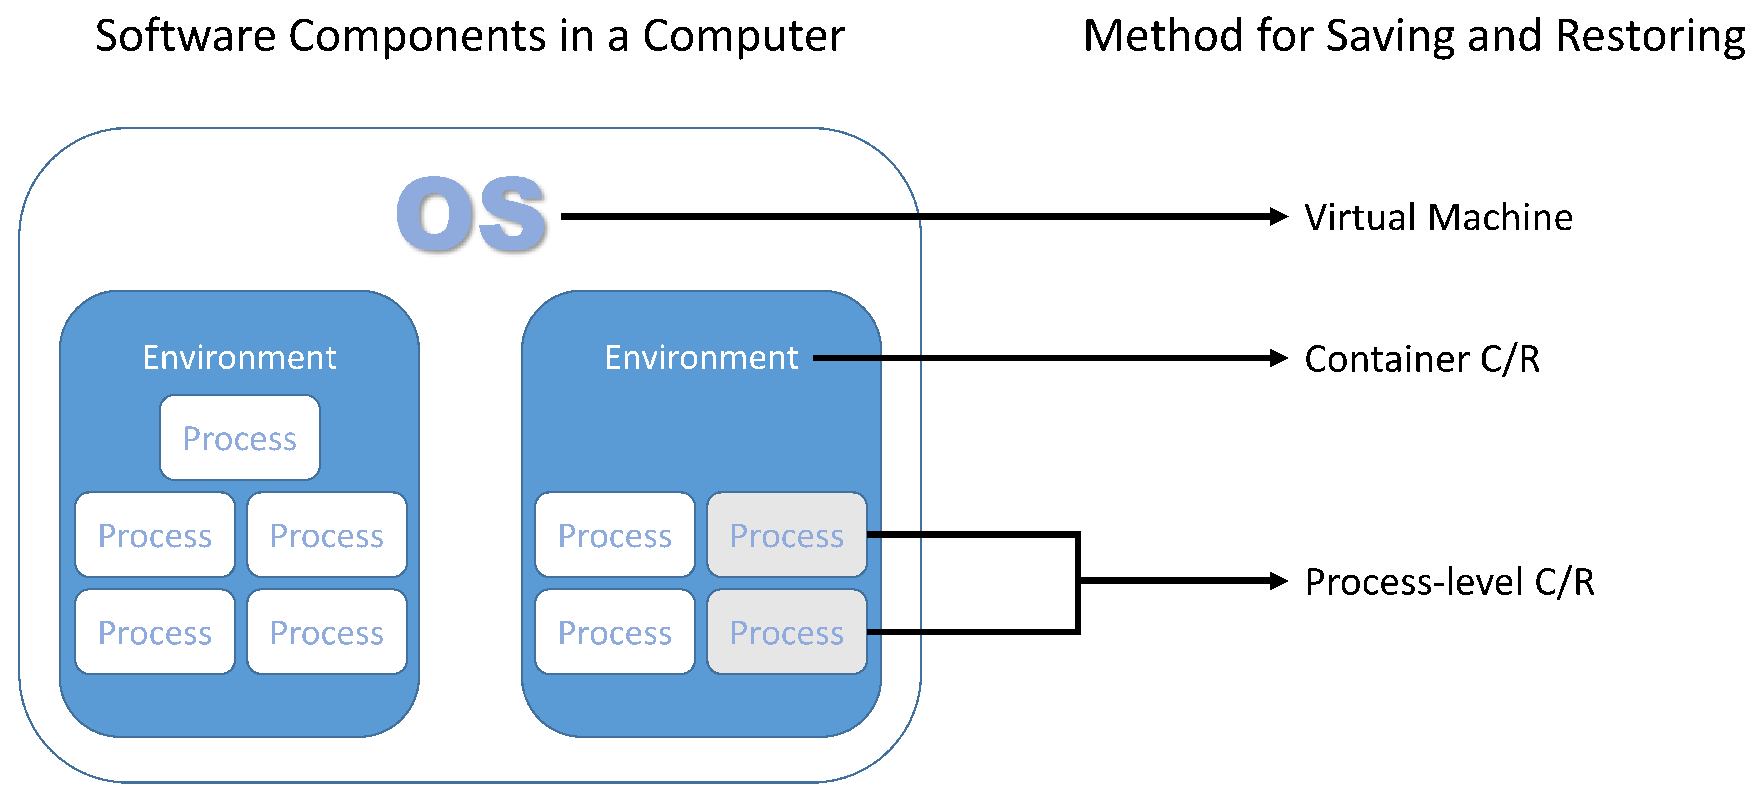
\includegraphics[width=13cm]{Types_of_CR}

\end{columns}
\end{frame}

%%%%%%%%%%%%%%%%%%%%%%%%%%%%%%%%%%%%%%%%%%%%%%%%%%%%%%%%%%%%%%%%%%%%%%%%%%%%%%%%%%%%%%%%%%

\begin{frame}
\frametitle{Virtual Machine (VM) C/R}
VM-level C/R is relatively easy to implement, once you have a VM: the
system is already isolated.
\begin{columns}[t]
\column{.5\textwidth}
\ul{\textit{Implementations}}
\begin{itemize}
\item Most any hypervisor platform: KVM, Virtualbox, VMWare, etc.
\item KVM is relatively lightweight; this is what we use on Red Cloud.
\end{itemize}

\ul{\textit{Pros}}
\begin{itemize}
\item Very simple to use.
\item Few suprises.
\item Many applications supported; few limitations.
\end{itemize}

\column{.5\textwidth}
\ul{\textit{Cons}}
\begin{itemize}
\item Operating in a VM context requires predefined partitioning of RAM and CPU
resources.
\item More overhead in most catgeories (storage of VM image, RAM snapshot, etc.).
\item Still a challenge for multi-VM C/R.
\end{itemize}

\end{columns}
\end{frame}
  
%%%%%%%%%%%%%%%%%%%%%%%%%%%%%%%%%%%%%%%%%%%%%%%%%%%%%%%%%%%%%%%%%%%%%%%%%%%%%%%%%%%%%%%%%%

\begin{frame}
\frametitle{Let's have a look at Virtual Box...}

{\only<1>{}}
{\only<2>{Note that all other solutions are currently Linux-dependent,
though some claim other UNIX systems could be \textit{easily}
supported.}}

\end{frame}

%%%%%%%%%%%%%%%%%%%%%%%%%%%%%%%%%%%%%%%%%%%%%%%%%%%%%%%%%%%%%%%%%%%%%%%%%%%%%%%%%%%%%%%%%%

\begin{frame}
\frametitle{Containers with C/R}
Containers are a form of virtualization that uses a single OS
kernel to run multiple, seemingly isolated, OS environments.
\begin{columns}[t]
\column{.5\textwidth}
\ul{\textit{Implementations}}
\begin{itemize}
\item \textbf{OpenVZ}
\item \textbf{CRIU} - Checkpoint/Restore In Userspace
\item Not all containers support C/R.
\end{itemize}

\ul{\textit{Pros}}
\begin{itemize}
\item Like VMs, enjoys the benefit of existing virtualization.
\item \textit{Fewer} suprises.
\end{itemize}

\column{.5\textwidth}
\ul{\textit{Cons}}
\begin{itemize}
\item \textit{May} incur additional overhead, due to C/R of
unnecessary processes and storage.
\item Still a challenge for multi-VM C/R.
\end{itemize}

\end{columns}

\end{frame}
  
%%%%%%%%%%%%%%%%%%%%%%%%%%%%%%%%%%%%%%%%%%%%%%%%%%%%%%%%%%%%%%%%%%%%%%%%%%%%%%%%%%%%%%%%%%

\begin{frame}
\frametitle{Kernel-modifying C/R}

Requires kernel modules or kernel patches to run.

\begin{columns}[t]
\column{.5\textwidth}
\ul{\textit{Implementations}}
\begin{itemize}
\item \textbf{OpenVZ}
\item \textbf{BLCR} - Berkeley Lab Checkpoint/Restart 
\item \textbf{\st{CRIU}} - But now in mainline!
\end{itemize}

\ul{\textit{Pros}}
\begin{itemize}
\item Varied.
\end{itemize}

\column{.5\textwidth}
\ul{\textit{Cons}}
\begin{itemize}
\item Requires modification of the kernel.
\item May not work for all kernels (BLCR does not past 3.7.1).
\end{itemize}

\end{columns}

\end{frame}
  
%%%%%%%%%%%%%%%%%%%%%%%%%%%%%%%%%%%%%%%%%%%%%%%%%%%%%%%%%%%%%%%%%%%%%%%%%%%%%%%%%%%%%%%%%%

\begin{frame}
\frametitle{Process-level C/R}

Checkpoint one or several interacting processes. Does not use the full container model.

\begin{columns}[t]
\column{.5\textwidth}
\ul{\textit{Implementations}}
\begin{itemize}
\item \textbf{BLCR}
\item \textbf{CRIU}
\item \textbf{DMTCP} - Distributed MultiThreaded CheckPointing
\end{itemize}

\ul{\textit{Pros}}
\begin{itemize}
\item Usually simple to use.
\item Lower overhead.
\end{itemize}

\column{.5\textwidth}
\ul{\textit{Cons}}
\begin{itemize}
\item May have surprises. Interesting apps use different
advanced feature sets (e.g. IPC), and each package
will have a different feature set. \textbf{Test first!}
\item BLCR requires modification of application for static linking.
\item CRIU is a bit new.
\end{itemize}

\end{columns}

% requires API

% versatile?


% left: Summary and implementations

% right: pros and cons 

\end{frame}
  
%%%%%%%%%%%%%%%%%%%%%%%%%%%%%%%%%%%%%%%%%%%%%%%%%%%%%%%%%%%%%%%%%%%%%%%%%%%%%%%%%%%%%%%%%%

\begin{frame}
\frametitle{Application-level C/R}

This is like ad-hoc, but when you do it even though you know
other C/R solutions exist.
\begin{columns}[t]
\column{.5\textwidth}
\ul{\textit{Libraries that help}}
\begin{itemize}
\item \textbf{(p)HDF5}
\item \textbf{NetCDF}
\end{itemize}

\ul{\textit{Pros}}
\begin{itemize}
\item Very low over-head.
\item Few surprises if done properly.
\end{itemize}

\column{.5\textwidth}
\ul{\textit{Cons}}
\begin{itemize}
\item Needs thorough testing for each app.
\item Lots of development time.
\item Less standardization.
\item Always a chance something is missed.
\end{itemize}

\end{columns}


\end{frame}

%%%%%%%%%%%%%%%%%%%%%%%%%%%%%%%%%%%%%%%%%%%%%%%%%%%%%%%%%%%%%%%%%%%%%%%%%%%%%%%%%%%%%%%%%%


%%%%%%%%%%%%%%%%%%%%%%%%%%%%%%%
                              %
\subsection{C/R For HPC}      %
                              %
%%%%%%%%%%%%%%%%%%%%%%%%%%%%%%%

%%%%%%%%%%%%%%%%%%%%%%%%%%%%%%%%%%%%%%%%%%%%%%%%%%%%%%%%%%%%%%%%%%%%%%%%%%%%%%%%%%%%%%%%%%

\begin{frame}
\frametitle{What is a good C/R solution for HPC?}

\begin{columns}[t]
\column{.5\textwidth}
\ul{\textit{Requirements}}
\begin{itemize}
\item Must be non-invasive.
  \begin{itemize}
  \item No kernel modifications.
  \item Preferably no libraries needed on nodes.
  \end{itemize}
\item Should have low overhead.
\item Must support distributed applications.
\end{itemize}

\column{.5\textwidth}
\ul{\textit{Bonuses}}
\begin{itemize}
\item Easy to use.
\item Stable for the user.
\end{itemize}

\end{columns}

\vspace{2ex}
It looks like DMTCP is the best candidate, for now.

% left: requirements (also add which solutions are precluded for each item)

% right: bonuses (no source modification/recompile), low overhead


\end{frame}

%%%%%%%%%%%%%%%%%%%%%%%%%%%%%%%%%%%%%%%%%%%%%%%%%%%%%%%%%%%%%%%%%%%%%%%%%%%%%%%%%%%%%%%%%%


%%%%%%%%%%%%%%%%%%%%%%%%%%%%%%%
%%%%%%%%%%%%%%%%%%%%%%%%%%%%%%%
                              %
\section{DMTCP}        %
                              %
%%%%%%%%%%%%%%%%%%%%%%%%%%%%%%%
%%%%%%%%%%%%%%%%%%%%%%%%%%%%%%%

%%%%%%%%%%%%%%%%%%%%%%%%%%%%%%%
                              %
\subsection{DMTCP Details}    % 
                              %
%%%%%%%%%%%%%%%%%%%%%%%%%%%%%%%

%%%%%%%%%%%%%%%%%%%%%%%%%%%%%%%%%%%%%%%%%%%%%%%%%%%%%%%%%%%%%%%%%%%%%%%%%%%%%%%%%%%%%%%%%%

\begin{frame}
\frametitle{An overview of DMTCP}

\begin{itemize}
\item Distributed MultiThreaded CheckPointing.
  \begin{itemize}
  \item Threads (OpenMP, POSIX threads), MPI.
  \end{itemize}
\item Easy to build and install library.
\item Not necessary to link with existing \ul{dynamically} linked
applications.
  \begin{itemize}
  \item DMTCP libs replace (wrap) standard libs and syscalls.
  \item DMTCP lib directory should be in \texttt{LD\_LIBRARY\_PATH} 
	\texttt{LD\_PRELOAD} (handled by DMTCP scripts).
  \end{itemize}
\item We are still evaluating; need to verify support for other MPI
implementations.
\end{itemize}

% stands for ...

% features, limitations

\end{frame}

%%%%%%%%%%%%%%%%%%%%%%%%%%%%%%%%%%%%%%%%%%%%%%%%%%%%%%%%%%%%%%%%%%%%%%%%%%%%%%%%%%%%%%%%%%

% \begin{frame}
% \frametitle{Configuring and installing DMTCP}


% \end{frame}

%%%%%%%%%%%%%%%%%%%%%%%%%%%%%%%%%%%%%%%%%%%%%%%%%%%%%%%%%%%%%%%%%%%%%%%%%%%%%%%%%%%%%%%%%%

%%%%%%%%%%%%%%%%%%%%%%%%%%%%%%%
                              %
\subsection{DMTCP examples}   % 
                              %
%%%%%%%%%%%%%%%%%%%%%%%%%%%%%%%

%%%%%%%%%%%%%%%%%%%%%%%%%%%%%%%%%%%%%%%%%%%%%%%%%%%%%%%%%%%%%%%%%%%%%%%%%%%%%%%%%%%%%%%%%%

\begin{frame}[fragile]
\frametitle{Counting in C}

\begin{columns}[t]
\column{.6\textwidth}

\begin{lstlisting}[basicstyle=\ttfamily, language=C, showstringspaces=false]

//Counting slowly

#include <stdio.h>
#include <unistd.h>

int main(void) {
  unsigned long i = 0;
  while (1) {
    printf("%lu ", i);
    i = i + 1;
    sleep(1);
    fflush(stdout);
  } 
} 

\end{lstlisting}

\column{.4\textwidth}

\begin{itemize}
\item \texttt{dmtcp\_checkpoint -i 5 ./count}
\item \texttt{dmtcp\_restart ckpt\_count\_xxx.dmtcp}
\end{itemize}

\end{columns}

\end{frame}

%%%%%%%%%%%%%%%%%%%%%%%%%%%%%%%%%%%%%%%%%%%%%%%%%%%%%%%%%%%%%%%%%%%%%%%%%%%%%%%%%%%%%%%%%%

\begin{frame}[fragile]
\frametitle{Counting in Perl}

\begin{columns}[t]
\column{.6\textwidth}

\begin{lstlisting}[basicstyle=\ttfamily, language=Perl, showstringspaces=false]

#Counting slowly

$| = 1; # autoflush STDOUT

$i = 0;
while (true) {
  print "$i ";
  $i = $i + 1;
  sleep(1);
}
\end{lstlisting}

\column{.4\textwidth}

\begin{itemize}
\item \texttt{dmtcp\_checkpoint -i 5 perl count.pl}
\item \texttt{dmtcp\_restart ckpt\_perl\_xxx.dmtcp}
\end{itemize}

\end{columns}


\end{frame}

%%%%%%%%%%%%%%%%%%%%%%%%%%%%%%%%%%%%%%%%%%%%%%%%%%%%%%%%%%%%%%%%%%%%%%%%%%%%%%%%%%%%%%%%%%

%%%%%%%%%%%%%%%%%%%%%%%%%%%%%%%
                              %
\subsection{Advanced DMTCP}   % 
                              %
%%%%%%%%%%%%%%%%%%%%%%%%%%%%%%%

\begin{frame}
\frametitle{X11 (graphics) support}

\begin{itemize}
\item All current non-VM C/R relies on VNC for X11 support.
\item DMTCP has a known bug with checkpointing \texttt{xterm}.
\item Due to dependence on VNC and general complications, only
try to use if you have to.
\end{itemize}
% Also mention BLCR and BLCR kernel caveat here?

\end{frame}


%%%%%%%%%%%%%%%%%%%%%%%%%%%%%%%%%%%%%%%%%%%%%%%%%%%%%%%%%%%%%%%%%%%%%%%%%%%%%%%%%%%%%%%%%%

\begin{frame}
\frametitle{Reversible Debugging with FReD}

\begin{itemize}
\item Supports GDB and several interpreters.
\item Allows you to inspect one part of the program, then
go back to a previous state without restarting the debugger.
\item \url{github.com/fred-dbg/fred}
\item \url{youtu.be/1l_wGZz0JEE}
\end{itemize}

\end{frame}

%%%%%%%%%%%%%%%%%%%%%%%%%%%%%%%%%%%%%%%%%%%%%%%%%%%%%%%%%%%%%%%%%%%%%%%%%%%%%%%%%%%%%%%%%%

\begin{frame}
\frametitle{DMTCP plugins}

\begin{block}{Used to modify the behavior of DMTCP}
Modify behavior at the time of checkpoint or restart.\\
\vspace{1ex}
Add wrapper functions around library functions (including syscalls).\\ 
\vspace{1ex}
Much of DMTCP itself is now written as plugins.\\
\vspace{1ex}
Custom plugins could add support for callbacks in user's program.\\
\end{block}

\end{frame}

%%%%%%%%%%%%%%%%%%%%%%%%%%%%%%%%%%%%%%%%%%%%%%%%%%%%%%%%%%%%%%%%%%%%%%%%%%%%%%%%%%%%%%%%%%



%%%%%%%%%%%%%%%%%%%%%%%%%%%%%%%%%%%%%%%%%%%%%%%%%%%%%%%%%%%%%%%%%%%%%%%%%%%%%%%%%%%%%%%%%%

%%%%%%%%%%%%%%%%%%%%%%%%%%%%%%%
%%%%%%%%%%%%%%%%%%%%%%%%%%%%%%%
                              %
\section{Closing}           %
                              %
%%%%%%%%%%%%%%%%%%%%%%%%%%%%%%%
%%%%%%%%%%%%%%%%%%%%%%%%%%%%%%%

%%%%%%%%%%%%%%%%%%%%%%%%%%%%%%%%%%%%%%%%%%%%%%%%%%%%%%%%%%%%%%%%%%%%%%%%%%%%%%%%%%%%%%%%%%

\subsection{Conclusions}
\begin{frame}
\frametitle{Conclusions}

\begin{itemize}
\item DMTCP appears to be good for most jobs for now. Also easy to install.
\item CRIU will likely be a strong contender in the future, but is not
yet ready for HPC.
\item BLCR and OpenVZ may be more robust than DMTCP for PID restoration (provided
your kernel has support for BLCR or OpenVZ).
\item For the foreseeable future, it is unlikely that any one C/R framework
will meet everyone's needs.


\end{itemize}

\end{frame}

%%%%%%%%%%%%%%%%%%%%%%%%%%%%%%%%%%%%%%%%%%%%%%%%%%%%%%%%%%%%%%%%%%%%%%%%%%%%%%%%%%%%%%%%%%

\subsection{Thank you!}
\begin{frame}
\frametitle{Thank you!} 

\begin{columns}[t]
%
\begin{column}{0.5\textwidth}
\ul{\textit{Additional Resources}}
\begin{itemize}
\item Slide source and other docs: \url{github.com/cornell-comp-internal/CR-demos}
\item FReD: \url{github.com/fred-dbg/fred}
\end{itemize}
\end{column}

\begin{column}{0.5\textwidth}
\ul{\textit{References}}
\begin{itemize}
\item Python and DMTCP: \url{youtu.be/1l_wGZz0JEE}
\item Comparison Chart: \url{criu.org/Comparison_to_other_CR_projects}
\end{itemize}

\vspace{0.4in}

% logo?

\end{column}

%
\end{columns}

\vspace{0.4in}
Questions? E-mail: \url{brandon.barker@cornell.edu}
\end{frame}

  


%%%%%%%%%%%%%%%%%%%%%%%%%%%%%%%%%%%%%%%%%%%%%%%%%%%%%%%%%%%%%%%%%%%%%%%%%%%%%%%%%%%%%%%%%%
%%%%%%%%%%%%%%%%%%%%%%%%%%%%%% End Your Document %%%%%%%%%%%%%%%%%%%%%%%%%%%%%%%%%%%%%%%%%
%%%%%%%%%%%%%%%%%%%%%%%%%%%%%%%%%%%%%%%%%%%%%%%%%%%%%%%%%%%%%%%%%%%%%%%%%%%%%%%%%%%%%%%%%%

\end{document}

